\documentclass{article}
\usepackage{amsmath}
\usepackage{graphicx} % Required for inserting images
\usepackage{enumerate}
\usepackage{ctex}
\usepackage{romannum}
\usepackage[colorlinks=true, allcolors=magenta]{hyperref}
\usepackage[legalpaper, margin=100pt]{geometry}
\usepackage{setspace}
\usepackage{tcolorbox}
\renewcommand{\baselinestretch}{1.25}

\setlength{\parindent}{20pt}

\title{第4章~曲面映射:度量}
\author{Wayne Zheng}
\date{\today}

\begin{document}

\maketitle

\section{度量}

\emph{度量}(Metric):也被称为第一基本形式(first fundamental form),表示两个临近点之间的无穷小距离的参数化规则。
参数化的规则选取可以有很多种,因此每个曲面原则上可以写下无穷多种度量。
度量决定了曲面的内蕴几何,这是高斯最早对微分几何的基本见解。

例如,平面可以有无穷多种度量,直角坐标系中$d\hat{s}^{2}=dx^{2}+dy^{2}$,极坐标中是$d\hat{s}^{2}=dr^{2}+r^{2}d\theta^{2}$.
其对应的\emph{度量张量}(metric tensor)分别为:
\begin{equation}
g=
\begin{pmatrix}
1 & 0 \\
0 & 1
\end{pmatrix}, \quad
g=
\begin{pmatrix}
1 & 0 \\
0 & r^{2}
\end{pmatrix}.
\end{equation}

\section{球面度量}

下面我们看球面的例子。
我们先考虑球坐标系$(\phi, \theta)$,其中$\phi\in[0, \pi]$是极角,表示纬度的取值范围;$\theta\in[0, 2\pi)$是方位角,表示经度的取值范围。
我们先来看几何直观。

\begin{figure}[htbp]
    \centering % 图片居中
    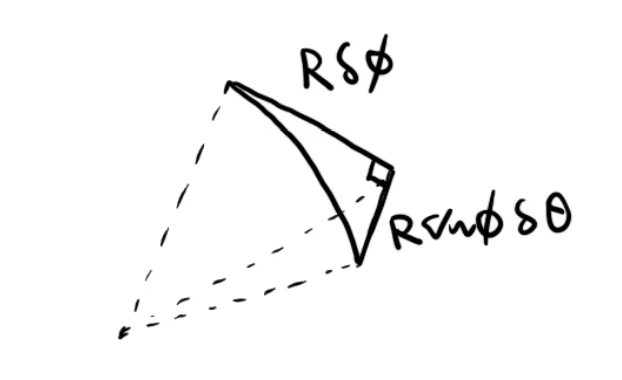
\includegraphics[width=0.3\textwidth]{../figs/chap4_01.jpg} % 图片路径
    \caption{球坐标系下的度量。} 
    \label{fig:chap4_01} 
\end{figure}

由图~\ref{fig:chap4_01}可知,球面上无穷小两点之间的距离可以表示为$d\hat{s}^{2}=\left(Rd\phi\right)^{2}+\left(R\sin\phi{d}\theta\right)^{2}$.


然后,让我们严格地详细计算这个度量。
球面上的一点$(x, y, z)$可以用球坐标参数化,即
\begin{equation*}
(x(\phi, \theta), y(\phi, \theta), z(\phi, \theta))=(R\sin\phi\cos\theta, R\sin\phi\sin\theta, R\cos\phi).
\end{equation*}
进一步地,球面上任意一条曲线可以用一个参数参数化,即$\mathbf{r}=\mathbf{r}(t)=\mathbf{r}(\phi(t), \theta(t))$.
其切向量为:$\mathbf{r}^{\prime}(t)=\partial_{\phi}\mathbf{r}\dot{\phi}+\partial_{\theta}\mathbf{r}\dot{\theta}$.
其中两个极坐标参数的切向量为:
\begin{equation}
\begin{aligned}
\mathbf{r}_{\phi}
&=\frac{\partial\mathbf{r}}{\partial\phi}
=\left(R\cos\phi\cos\theta, R\cos\phi\sin\theta, -R\sin\phi\right), \\
\mathbf{r}_{\theta}
&=\frac{\partial\mathbf{r}}{\partial\theta}
=\left(-R\sin\phi\sin\theta, R\sin\phi\cos\theta, 0\right).
\end{aligned}
\end{equation}
球面度量为
\begin{equation*}
\begin{aligned}
d\hat{s}^{2}
&=dx^{2}+dy^{2}+dz^{2} \\
&=\left(\partial_{\phi}{x}d\phi+\partial_{\theta}{x}d\theta\right)^{2}+\left(\partial_{\phi}{y}d\phi+\partial_{\theta}{y}d\theta\right)^{2}+\left(\partial_{\phi}{z}d\phi+\partial_{\theta}{z}d\theta\right)^{2} \\
&=\mathbf{r}_{\phi}\cdot\mathbf{r}_{\phi}d\phi^{2}+\mathbf{r}_{\theta}\cdot\mathbf{r}_{\theta}d\theta^{2}+\mathbf{r}_{\phi}\cdot\mathbf{r}_{\theta}d\phi{d}\theta+\mathbf{r}_{\theta}\cdot\mathbf{r}_{\phi}d\theta{d}\phi.
\end{aligned}
\end{equation*}
则其度量张量为
\begin{equation}
g=\begin{pmatrix}
g_{\phi\phi} & g_{\phi\theta} \\
g_{\theta\phi} & g_{\theta\theta}
\end{pmatrix}
=\begin{pmatrix}
\mathbf{r}_{\phi}\cdot\mathbf{r}_{\phi} & \mathbf{r}_{\phi}\cdot\mathbf{r}_{\theta} \\
\mathbf{r}_{\theta}\cdot\mathbf{r}_{\phi} & \mathbf{r}_{\theta}\cdot\mathbf{r}_{\theta}
\end{pmatrix}
=\begin{pmatrix}
R^{2} & 0 \\
0 & R^{2}\sin^{2}\phi
\end{pmatrix}.
\end{equation}
最终,球面用$(\phi, \theta)$写下的度量为$d\hat{s}^{2}=R^{2}\left(d\phi^{2}+\sin^{2}\phi{d}\theta^{2}\right)$,与几何直观方法得到的一致。

类似地,我们计算中心投影的度量(习题3)。首先是用切平面上的参数$(r, \theta)$来参数化球面上的点:
\begin{equation*}
\begin{aligned}
\mathbf{l}=(x, y, z)
&=(R\sin\phi\cos\theta, R\sin\phi\sin\theta, R\cos\phi) \\
&=\left(\frac{Rr\cos\theta}{\sqrt{R^{2}+r^{2}}}, \frac{Rr\sin\theta}{\sqrt{R^{2}+r^{2}}}, \frac{R^{2}}{\sqrt{R^{2}+r^{2}}}\right).
\end{aligned}
\end{equation*}
相应地,可以计算切向量$\mathbf{l}_{r}=\partial_{r}\mathbf{l}, \mathbf{l}_\theta=\partial_{\theta}\mathbf{l}$.
度量张量为
\begin{equation}
g=\begin{pmatrix}
g_{r\phi} & g_{r\theta} \\
g_{\theta{r}} & g_{\theta\theta}
\end{pmatrix}
=\begin{pmatrix}
\mathbf{l}_{r}\cdot\mathbf{l}_{r} & \mathbf{l}_{r}\cdot\mathbf{l}_{\theta} \\
\mathbf{l}_{\theta}\cdot\mathbf{l}_{r} & \mathbf{l}_{\theta}\cdot\mathbf{l}_{\theta}
\end{pmatrix}
=\begin{pmatrix}
\frac{R^{4}}{\left(R^{2} + r^{2}\right)^{2}} & 0 \\
0 & \frac{R^{2}r^{2}}{R^{2} + r^{2}}
\end{pmatrix}.
\end{equation}
则其度量为
\begin{equation}
d\hat{s}^{2}=\frac{R^{4}}{\left(R^{2}+r^{2}\right)^{2}}dr^{2}+\frac{R^{2}r^{2}}{R^{2}+r^{2}}d\theta^{2}
=\frac{1}{1+(r/R)^{2}}\left[\frac{dr^{2}}{1+(r/R)^{2}}+r^{2}d\theta^{2}\right],
\end{equation}
与几何直观方法得到的一致。

\begin{figure}[htbp]
    \centering % 图片居中
    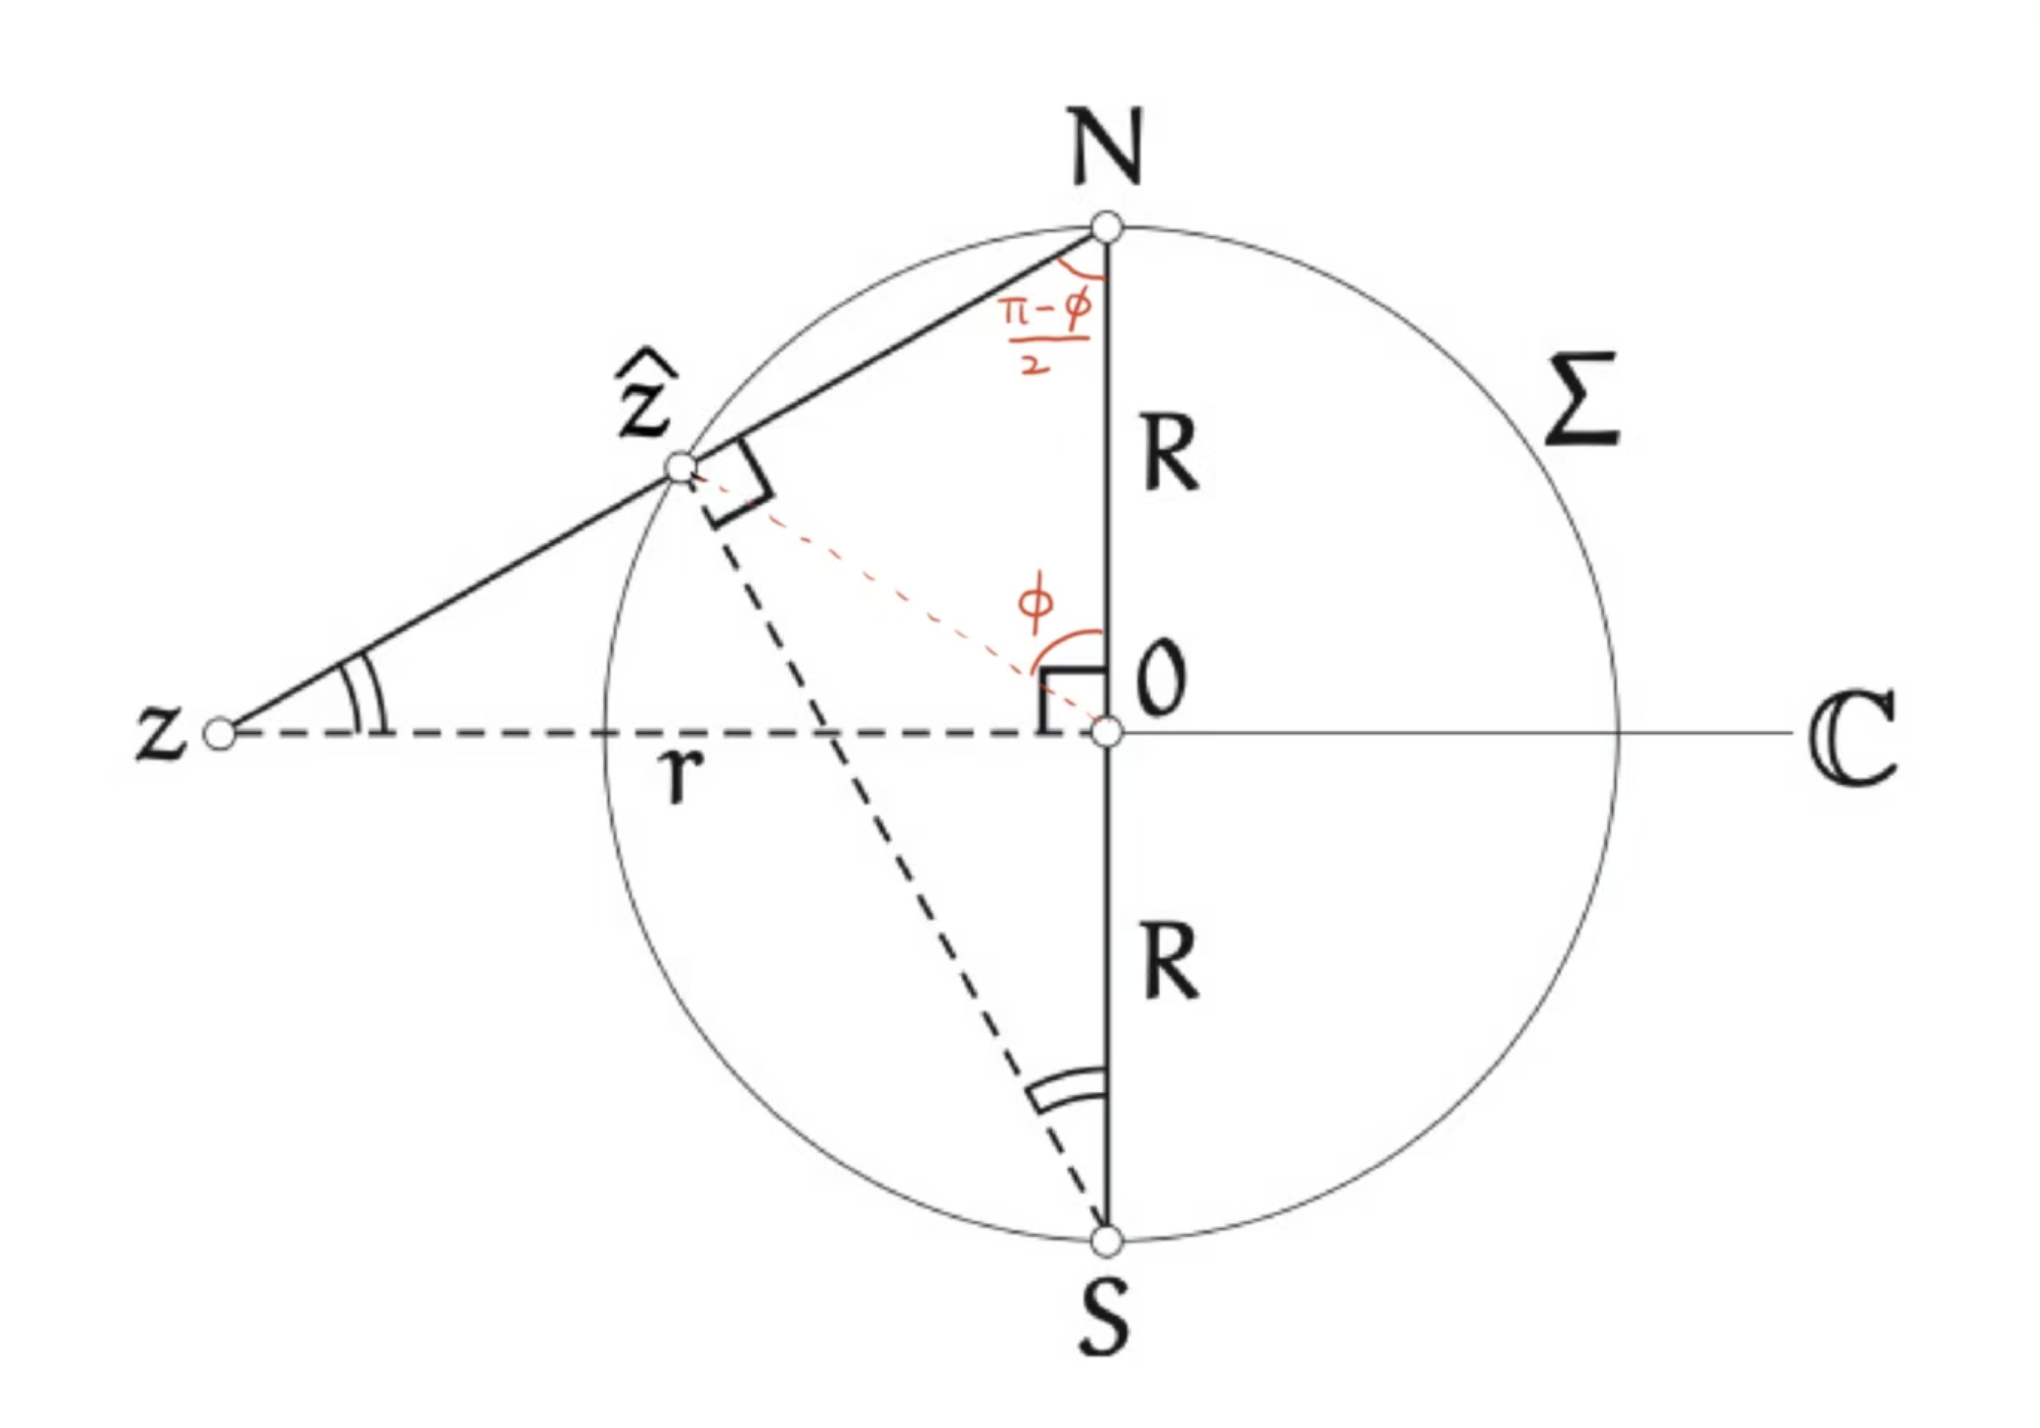
\includegraphics[width=0.5\textwidth]{../figs/chap4_02.png}
    \caption{球极投影的侧剖图。} 
    \label{fig:chap4_02} 
\end{figure}

我们再来计算球极投影的度量。
如图~\ref{fig:chap4_02}所示,我们有:
\begin{equation*}
\sin\left(\frac{\pi-\phi}{2}\right)
=\cos\left(\frac{\phi}{2}\right)=\frac{r}{\sqrt{R^{2}+r^{2}}}, \quad
\cos\left(\frac{\pi-\phi}{2}\right)
=\sin\left(\frac{\phi}{2}\right)=\frac{R}{\sqrt{R^{2}+r^{2}}}.
\end{equation*}
球极投影的参数化为
\begin{equation*}
\begin{aligned}
\mathbf{l}=(x, y, z)
&=(R\sin\phi\cos\theta, R\sin\phi\sin\theta, R\cos\phi) \\
&=\left[\frac{2R^{2}r\cos\theta}{R^{2}+r^{2}}, \frac{2R^{2}r\sin\theta}{R^{2}+r^{2}}, \frac{R(r^{2}-R^{2})}{R^{2}+r^{2}}\right].
\end{aligned}
\end{equation*}
相应地,可以计算切向量$\mathbf{l}_{r}=\partial_{r}\mathbf{l}, \mathbf{l}_\theta=\partial_{\theta}\mathbf{l}$.
度量张量为
\begin{equation}
g=\begin{pmatrix}
g_{r\phi} & g_{r\theta} \\
g_{\theta{r}} & g_{\theta\theta}
\end{pmatrix}
=\begin{pmatrix}
\mathbf{l}_{r}\cdot\mathbf{l}_{r} & \mathbf{l}_{r}\cdot\mathbf{l}_{\theta} \\
\mathbf{l}_{\theta}\cdot\mathbf{l}_{r} & \mathbf{l}_{\theta}\cdot\mathbf{l}_{\theta}
\end{pmatrix}
=\begin{bmatrix}
\frac{4R^{4}}{\left(R^{2} + r^{2}\right)^{2}} & 0 \\
0 & \frac{4R^{4}r^{2}}{\left(R^{2} + r^{2}\right)^{2}}
\end{bmatrix}.
\end{equation}
则其度量为$d\hat{s}^{2}=\frac{4R^{4}}{\left(R^{2} + r^{2}\right)^{2}}\left(dr^{2}+r^{2}d\theta^{2}\right)$.
即$d\hat{s}=\frac{2R^{2}}{R^{2} + r^{2}}ds$,是一个共形变换,与几何直观方法得到的一致。

\section{球极投影的保圆性}

\begin{tcolorbox}[colback=white, arc=3mm, auto outer arc]
\begin{minipage}[c,t]{1.0\textwidth}
\kaishu
设平面的方程为:
\begin{equation*}
    Ax+By+Cz=D.
\end{equation*}
设$P=(x_{0}, y_{0}, z_{0})$ 与$Q=(x_{1}, y_{1}, z_{1})$是平面上的两点,$\mathbf{v}\equiv(x_{1}-x_{0}, y_{1}-y_{0}, z_{1}-z_{0})$.
则显然$\mathbf{v}$与$\mathbf{n}=(A, B, C)$正交,即$\mathbf{v}\cdot\mathbf{n}=0$.
$\mathbf{n}$是平面的法向量。
另设$P^{\prime}=(x_{0}^{\prime}, y_{0}^{\prime}, z_{0}^{\prime})$是平面外的任意一点,则$P^{\prime}$到平面的距离的向量即为投影到法向量方向:$    \mathbf{d}=\text{Proj}_{\mathbf{n}}\left(\overrightarrow{P^{\prime}P}\right)=\vert\overrightarrow{P^{\prime}P}\vert\cos\alpha\hat{\mathbf{n}}$.
距离为
\begin{equation*}
d=\overrightarrow{P^{\prime}P}\cdot\hat{\mathbf{n}}
=\frac{\vert Ax_{0}^{\prime}+By_{0}^{\prime}+Cz_{0}^{\prime}-D\vert}{\sqrt{A^{2}+B^{2}+C^{2}}}.
\end{equation*}
\end{minipage}
\end{tcolorbox}

%\bibliographystyle{unsrt}
%\bibliography{refs}
\end{document}